\chapter{Neural Networks as Markov Chains}

% 1. Descriptive Opening
Deep neural networks are often conceptualized as complex, non-linear function approximators, iteratively refining an input signal to produce a desired output. However, through the lens of information theory, a neural network is best understood as a sequence of random variables forming a Markov chain. As data propagates from the input layer through successive hidden layers to the final output, it undergoes a series of stochastic or deterministic transformations. This perspective fundamentally shifts our understanding: rather than merely computing features, each layer acts as a filter that selectively discards irrelevant information while retaining what is necessary for the task at hand.

When we observe an input $X \in \mathcal{X}$, such as an image or a sentence, it is intrinsically tied to a target variable $Y \in \mathcal{Y}$, which we wish to predict. The input $X$ is fed into the network, producing a first-layer representation $T_1$. This representation $T_1$ is then processed to create $T_2$, and so on, up to the final layer $T_L$, which is used to generate the prediction $\hat{Y}$. Because the computation of any layer $T_i$ depends strictly on the output of the immediately preceding layer $T_{i-1}$ (along with the network parameters), the sequence of representations forms a Markov chain.

The implications of this Markovian structure are profound. It imposes strict bounds on the flow of information through the network. According to the laws of information theory, post-processing a signal cannot increase its information content. Every layer, at best, perfectly preserves the information about the input and the target, but in most practical architectures, information is strictly lost. This progressive loss of information is not a flaw; rather, it is the very essence of abstraction. By shedding nuisance factors---the exact pixel values, the background noise, the variations in lighting---the network distills the input down to its most invariant and predictive features. 

Understanding neural networks as Markov chains allows us to rigorously quantify the concepts of representation learning, feature extraction, and abstraction. It provides the theoretical scaffolding to ask precise questions: How much information does a specific layer retain about the input? How much information does it retain about the target? And how does this balance dictate the network's ability to generalize to unseen data?

% 2. Mathematical Core
\section{The Markovian Structure of Deep Networks}

To formalize this perspective, let us consider a feedforward neural network. Let $X$ be the random variable representing the input data, and $Y$ be the corresponding true label. The network consists of $L$ hidden layers, which we denote as a sequence of random variables $T_1, T_2, \ldots, T_L$. 

Recall from \cref{ch:mutual_information} that a sequence of random variables forms a Markov chain if the future is conditionally independent of the past given the present state. 

In a standard feedforward neural network, the mapping from $T_{i-1}$ to $T_i$ is typically deterministic, parameterized by weights and biases $\theta_i$, and followed by a non-linear activation function. If we consider stochastic networks (e.g., with dropout, additive noise, or stochastic activations), the mapping becomes explicitly probabilistic. Even in deterministic networks, $T_i$ is a deterministic function of $T_{i-1}$, meaning the conditional entropy $H(T_i \mid T_{i-1}) = 0$. In either case, the Markov property holds.

Thus, the entire supervised learning setup can be described by the following Markov chain:
\[ Y \leftrightarrow X \leftrightarrow T_1 \leftrightarrow T_2 \leftrightarrow \cdots \leftrightarrow T_L \leftrightarrow \hat{Y} \]
The relation $Y \leftrightarrow X$ implies that the true label $Y$ and the observation $X$ are jointly distributed according to the true data distribution $P_{\text{data}}(X, Y)$. The network only has access to $X$, not $Y$, when computing the representations.

\begin{figure}[ht]
\centering
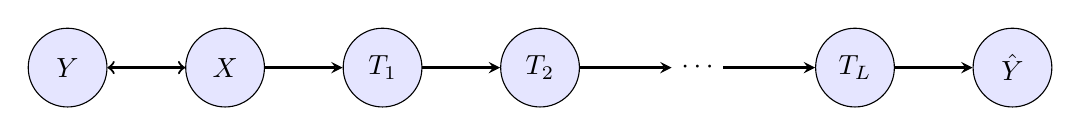
\begin{tikzpicture}[
    node distance=2cm,
    var/.style={circle, draw, minimum size=1cm, fill=blue!10},
    arrow/.style={-stealth, thick}
]
    \node[var] (Y) {$Y$};
    \node[var, right of=Y] (X) {$X$};
    \node[var, right of=X] (T1) {$T_1$};
    \node[var, right of=T1] (T2) {$T_2$};
    \node[right of=T2] (dots) {$\cdots$};
    \node[var, right of=dots] (TL) {$T_L$};
    \node[var, right of=TL] (Yhat) {$\hat{Y}$};

    \draw[<->, thick] (Y) -- (X);
    \draw[arrow] (X) -- (T1);
    \draw[arrow] (T1) -- (T2);
    \draw[arrow] (T2) -- (dots);
    \draw[arrow] (dots) -- (TL);
    \draw[arrow] (TL) -- (Yhat);
\end{tikzpicture}
\caption{The Markov chain representing the flow of information in a feedforward neural network.}
\label{fig:nn_markov}
\end{figure}

\section{The Data Processing Inequality (DPI)}

The most critical consequence of the Markov chain structure is the Data Processing Inequality (DPI). The DPI states that no local processing of data can increase the amount of information it contains.

As established in \cref{thm:dpi}, this principle dictates that post-processing cannot generate new information. We recall the result here: if $X \leftrightarrow Y \leftrightarrow Z$ forms a Markov chain, then $I(X; Z) \le I(X; Y)$. The formal proof, which relies on the chain rule for mutual information and conditional independence, was detailed in \cref{ch:mutual_information}.

Applying the DPI to our neural network Markov chain $Y \leftrightarrow X \leftrightarrow T_1 \leftrightarrow \cdots \leftrightarrow T_L$, we obtain a sequence of inequalities for the mutual information with respect to both the input $X$ and the target $Y$.

\begin{corollary}[Monotonicity of Information in Neural Networks]
For a neural network forming the Markov chain $Y \leftrightarrow X \leftrightarrow T_1 \leftrightarrow \cdots \leftrightarrow T_L$, the information about the input monotonically decreases (or remains constant) across layers:
\[ I(X; X) \ge I(X; T_1) \ge I(X; T_2) \ge \cdots \ge I(X; T_L) \]
Similarly, the information about the target monotonically decreases:
\[ I(Y; X) \ge I(Y; T_1) \ge I(Y; T_2) \ge \cdots \ge I(Y; T_L) \]
\end{corollary}

This corollary mathematically crystallizes the concept of abstraction. As the data progresses through the network, the layers systematically discard information about the input $X$. Ideally, the network sheds the nuisance information (i.e., information in $X$ that is irrelevant to $Y$) while preserving the predictive information $I(Y; T_i)$. 

\begin{figure}[ht]
\centering
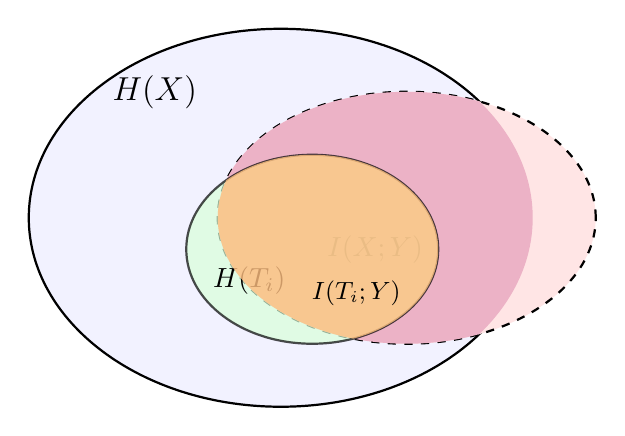
\begin{tikzpicture}[scale=0.8]
    % Outer set X
    \draw[thick, fill=blue!5] (0,0) ellipse (4cm and 3cm);
    \node at (-2, 2) {\large $H(X)$};
    
    % Target set Y
    \draw[thick, fill=red!10, dashed] (2,0) ellipse (3cm and 2cm);
    \node at (3, 1) {\large $H(Y)$};
    
    % Intersection representing I(X; Y)
    \begin{scope}
        \clip (0,0) ellipse (4cm and 3cm);
        \fill[purple!30] (2,0) ellipse (3cm and 2cm);
    \end{scope}
    \node at (1.5, -0.5) {$I(X;Y)$};

    % Layer T_i
    \draw[thick, fill=green!15, opacity=0.7] (0.5, -0.5) ellipse (2cm and 1.5cm);
    \node at (-0.5, -1) {$H(T_i)$};
    
    % T_i intersection with I(X;Y)
    \begin{scope}
        \clip (0.5, -0.5) ellipse (2cm and 1.5cm);
        \clip (0,0) ellipse (4cm and 3cm);
        \fill[orange!50, opacity=0.8] (2,0) ellipse (3cm and 2cm);
    \end{scope}
    \node at (1.2, -1.2) {\small $I(T_i; Y)$};
\end{tikzpicture}
\caption{Information Venn Diagram. The representation $T_i$ can only capture a subset of the information that $X$ contains about $Y$, bounded by the Data Processing Inequality.}
\label{fig:venn_dpi}
\end{figure}

\section{Numerical Example: Linear Additive Gaussian Noise}
To illustrate the progressive loss of information, consider a simple Markov chain model where each layer applies a linear scaling followed by additive Gaussian noise. Let the input $X \sim \mathcal{N}(0, \sigma_X^2)$.
The first layer is $T_1 = a_1 X + Z_1$, where $Z_1 \sim \mathcal{N}(0, \sigma_1^2)$ is independent of $X$.
The second layer is $T_2 = a_2 T_1 + Z_2$, where $Z_2 \sim \mathcal{N}(0, \sigma_2^2)$ is independent of $T_1$ and $X$.

We wish to compute $I(X; T_1)$ and $I(X; T_2)$ to observe the DPI in action.

First, the mutual information between continuous Gaussian variables depends on their differential entropy. The mutual information is $I(X; T_1) = \frac{1}{2} \log(1 + \text{SNR}_1)$, where the Signal-to-Noise Ratio is $\text{SNR}_1 = \frac{a_1^2 \sigma_X^2}{\sigma_1^2}$. Thus:
\[ I(X; T_1) = \frac{1}{2} \log\left( 1 + \frac{a_1^2 \sigma_X^2}{\sigma_1^2} \right) \]

For the second layer, we express $T_2$ directly in terms of $X$:
\[ T_2 = a_2 (a_1 X + Z_1) + Z_2 = a_2 a_1 X + a_2 Z_1 + Z_2 \]
The effective signal variance is $(a_2 a_1)^2 \sigma_X^2$.
The effective noise is $Z_{\text{eff}} = a_2 Z_1 + Z_2$, which has variance $a_2^2 \sigma_1^2 + \sigma_2^2$.
The mutual information is:
\[ I(X; T_2) = \frac{1}{2} \log\left( 1 + \frac{a_1^2 a_2^2 \sigma_X^2}{a_2^2 \sigma_1^2 + \sigma_2^2} \right) \]

To verify $I(X; T_2) \le I(X; T_1)$, observe the argument of the logarithm for $T_2$:
\[ \frac{a_1^2 a_2^2 \sigma_X^2}{a_2^2 \sigma_1^2 + \sigma_2^2} = \frac{a_1^2 \sigma_X^2}{\sigma_1^2 + \frac{\sigma_2^2}{a_2^2}} \le \frac{a_1^2 \sigma_X^2}{\sigma_1^2} \]
Since the noise term $\frac{\sigma_2^2}{a_2^2}$ is strictly non-negative, the SNR strictly decreases (unless $\sigma_2^2 = 0$, representing no noise), implying $I(X; T_2) \le I(X; T_1)$. The addition of independent noise at each processing step irrevocably destroys information.

% 3. Horizon Box
\begin{horizon}
While the Data Processing Inequality dictates that information must monotonically decrease through a strictly sequential Markov chain, the architectural reality of modern deep learning is far more complex. It is conjectured that the extraordinary success of architectures like ResNets and Transformers stems fundamentally from their ability to bypass strict Markovian bottlenecks. By utilizing residual connections ($T_{i+1} = T_i + f(T_i)$) or dense attention mechanisms, these models route information outside the sequential chain, creating a directed acyclic graph rather than a simple line. 

An open question is how to rigorously track mutual information bounds in these non-Markovian graphs. Does the network selectively filter information across skip connections, or do these connections merely delay the inevitable compression phase? Furthermore, in continuous-depth models such as Neural ODEs, layers are replaced by a continuous time variable $t$. Future work might show that the evolution of mutual information $I(X; T(t))$ in these systems is governed by a diffusion-like differential equation, extending the DPI from discrete jumps to a continuous flow. 

To close this theoretical gap, we would need robust, scalable estimators for high-dimensional mutual information that can operate over the computational graphs of modern architectures. If such estimators were developed, we might be able to definitively prove whether extreme depth inherently enforces optimal compression, or if architectural "shortcuts" allow networks to cheat the bottleneck entirely.
\end{horizon}

% 4. Summary + Exercises
\section*{Summary}
In this chapter, we framed deep neural networks as Markov chains, establishing that the sequential processing of data inherently limits information flow. We rigorously defined the Data Processing Inequality (DPI) and proved that both the information retained about the input and the information predictive of the target must monotonically decrease as data moves deeper into the network. This mathematical framework demystifies representation learning, showing that abstract features are forged by the unavoidable loss of nuisance information through successive transformations.

\section*{Exercises}
\begin{enumerate}
    \item \textbf{Invertible Networks:} Consider a neural network where every layer $T_i$ is a bijective (invertible) function of $T_{i-1}$, such as in a Normalizing Flow. Prove that for all $i \in \{1, \ldots, L\}$, $I(X; T_i) = I(X; X)$. What does this imply about the abstraction capabilities of strictly invertible networks?
    \item \textbf{Conditional DPI:} Prove the conditional version of the Data Processing Inequality. If $X \leftrightarrow Y \leftrightarrow Z$ forms a Markov chain, show that for any other random variable $W$, it holds that $I(X; Z \mid W) \le I(X; Y \mid W)$ provided $X \leftrightarrow Y \leftrightarrow Z$ remains a Markov chain when conditioned on $W$.
    \item \textbf{Information Paths:} Let a network have a single skip connection such that $T_2 = f(T_1, X)$. Draw the corresponding causal graph. Does the sequence $X \leftrightarrow T_1 \leftrightarrow T_2$ still form a Markov chain? Explain whether $I(X; T_2) \le I(X; T_1)$ is necessarily true in this architecture.
\end{enumerate}

% TODO-CITE: Ensure all named results are cited.
